\subsection{Priklausomybių versijavimas Go sistemoje}

Go inžinierių pasiūlymas dėl version-aware Go komandos implementacijos apsprendžia, kaip naujoje
Go bus versijuojamos priklausomybės. Trečiasis šio pasiūlymo punktas nurodo, kad atnaujintoje Go bus
naudojamas semantinis importų versijavimas (ang. semantic import versioning) \cite{COX18c}.
Semantiniu importų versijavimu siekiama, jog su kiekvienam atgaliai nesuderinamui paketo pakeitimui bus priskiriamas
skirtingas importavimo kelias (ang. import path) su specifikuota pagrindine (ang. major) versija, pavyzdžiui, “github.com/greta/foo/v2".

\begin{figure}[H]
    \centering
    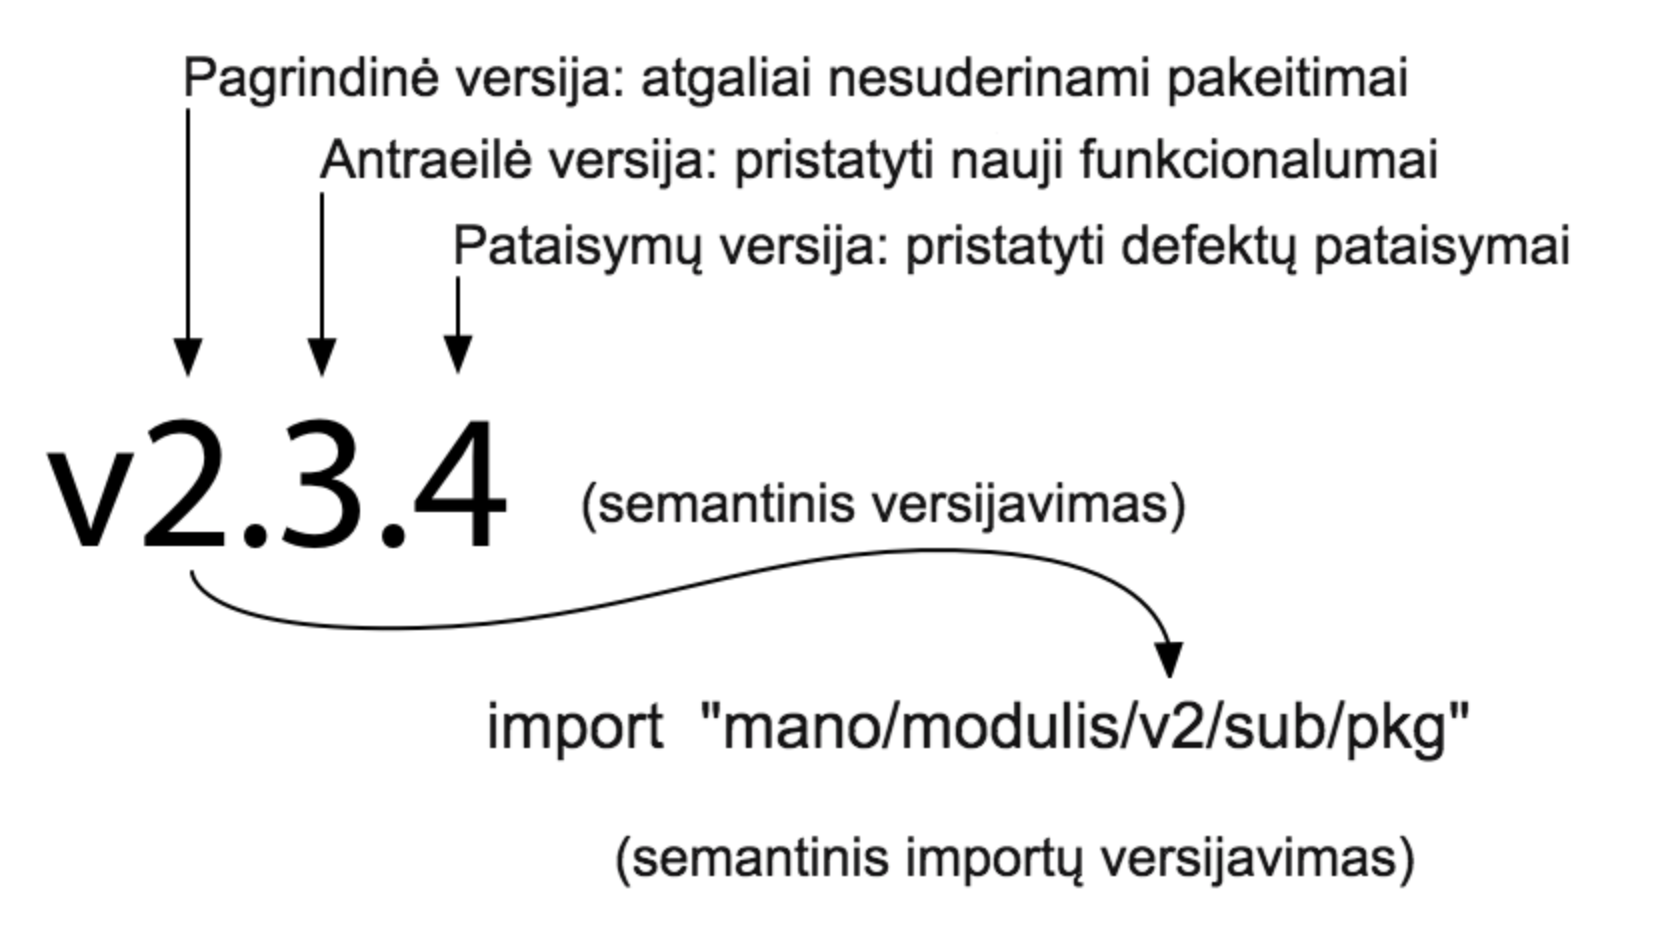
\includegraphics[width=\textwidth]{imp_semver2}
    \caption{Semantinis importų versijavimas \cite{COX18d}}
\end{figure}

Ketvirtasis Go pasiūlymo punktas, importų suderinamumo taisyklė, papildo prieš
tai pasiūlyme pristatytą semantinio importų versijavimo idėją. Ši taisyklė teigia: jei
senas paketas ir naujas paketas turi tą patį importavimo kelią, tuomet naujas paketas privalo būti atgaliai
suderinamas su senuoju \cite{COX18c}. Importų suderinamumo taisyklė paketų autoriams nustato griežtas ribas, kokie pakeitimai leidžiami
nekeičiant paketo importavimo kelio ir kokius pakeitimus įvykdžius būtina kurti naują importavimo kelią.

Naudojant semantinį paketų versijavimą bei laikantis importų suderinamumo taisyklės tikimasi išspręsti prieš tai „go get“
komandoje buvusią nestabilaus API problemą - paketų naudotojams suteikiama garantija,
kad atnaujinant priklausomybes jų naudojamų paketų metodai nesikeis.
